\section{Конструкторская часть}

\subsection{Описание команд}
В соответствии с выделенным в предыдущем разделе функционалом, в качестве необходимых для взаимодействия с устройством выделим команды, указанные в таблице \ref{tab:commands} (с указанием их аргументов и возвращаемого значения):
\begin{table}[h] 
	\caption{Команды ввода/вывода}
	\label{tab:commands}
	\begin{tabular}{| X | X | X |}
		\hline
		
		\textbf{Команда} &
		\textbf{Аргументы} &
		\textbf{Возвращаемое значение} \\ \hline
		
		Чтение	&	
		№ пина  &
		Значение пина \\ \hline
		
		Запись	&	
		№ пина, значение  &
		- \\ \hline
		
		Переключение &	
		№ пина  &
		Значение пина \\ \hline
		
		Установка / Сброс &	
		№ пина  &
		- \\ \hline
		
		Захват владения &	
		№ пина  &
		- \\ \hline
		
		Освобождение владения &	
		№ пина  &
		- \\ \hline
		
		Установка режима &	
		№ пина, режим  &
		- \\ \hline
	\end{tabular}
\end{table}

Также для демонстрации работы данных команд необходимо разработать программу пользовательского уровня. Она должна предоставлять интерфейс для выбора команды, ввода её аргументов и отображения результата выполнения операции ввода/вывода.


\subsection{Алгоритм обработки команды}
На рисунке \ref{alg:command} приведён алгоритм обработки команды ввода/вывода.
\begin{figure}[h!] 
	\begin{center}
		{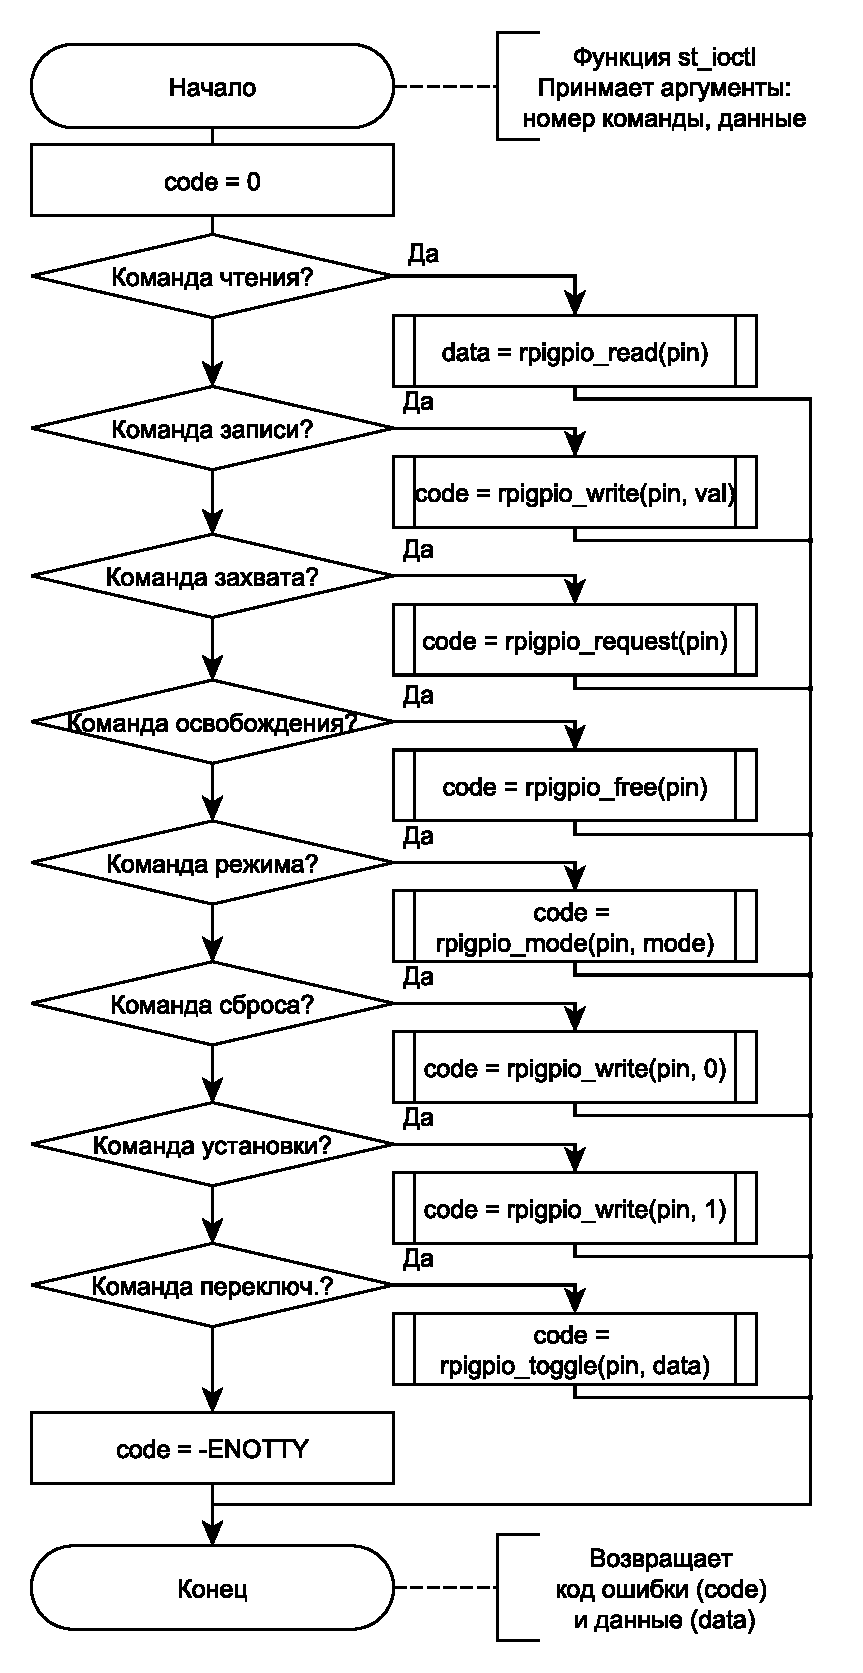
\includegraphics[scale=0.7, angle=0]{img/command.pdf}}
		\caption{Алгоритм обработки команды}
		\label{alg:command}
	\end{center}
\end{figure}
\pagebreak

\subsection{Алгоритмы чтения/записи значения}
На рисунках \ref{alg:read}, \ref{alg:write} и \ref{alg:toggle} приведены алгоритмы чтения, записи и переключения значения контакта соотвественно.
\begin{figure}[h!] 
	\begin{center}
		{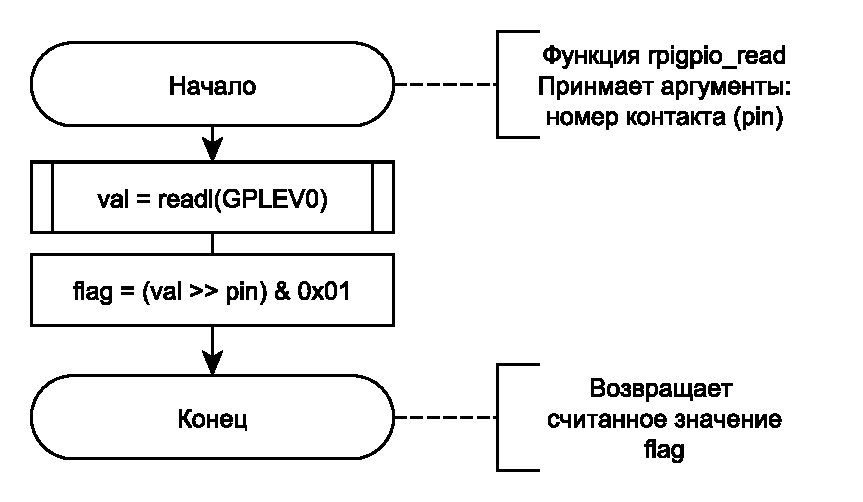
\includegraphics[scale=0.7, angle=0]{img/read.pdf}}
		\caption{Алгоритм чтения значения}
		\label{alg:read}
	\end{center}
\end{figure}

\begin{figure}[h!] 
	\begin{center}
		{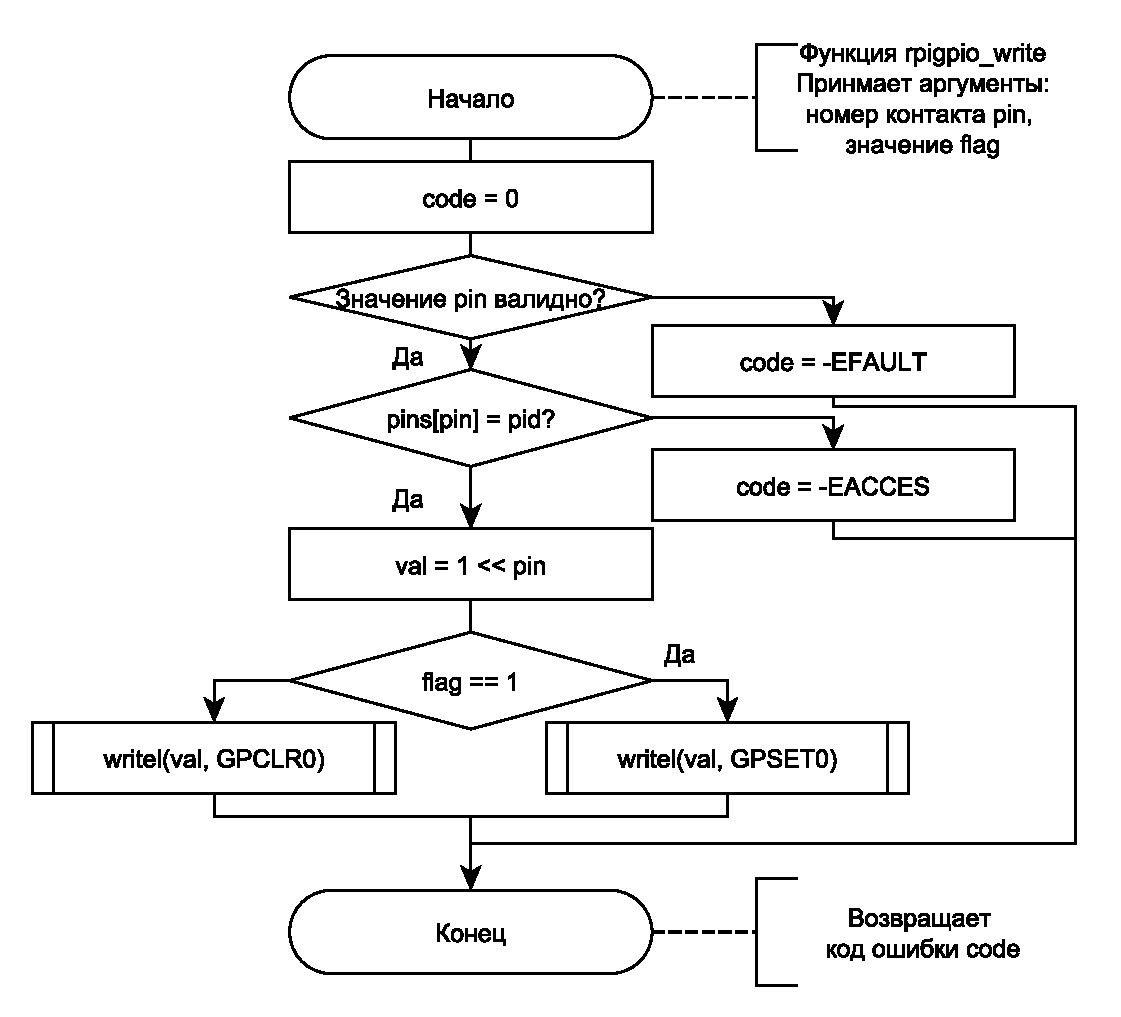
\includegraphics[scale=0.7, angle=0]{img/write.pdf}}
		\caption{Алгоритм установки значения}
		\label{alg:write}
	\end{center}
\end{figure}

\begin{figure}[h!] 
	\begin{center}
		{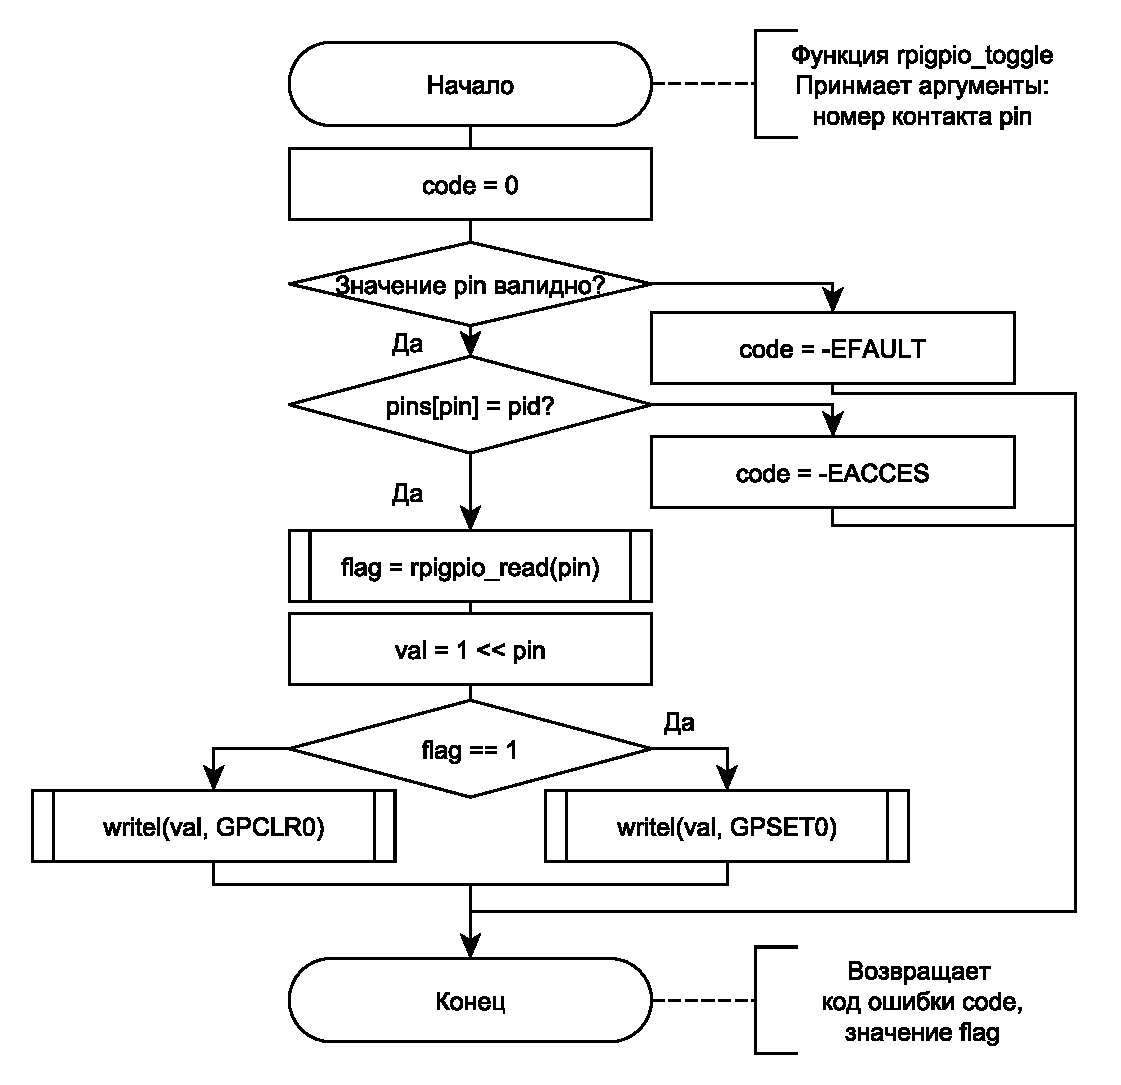
\includegraphics[scale=0.7, angle=0]{img/toggle.pdf}}
		\caption{Алгоритм переключения значения}
		\label{alg:toggle}
	\end{center}
\end{figure}

\subsection{Алгоритмы захвата/освобождения}
На рисунках \ref{alg:read}, \ref{alg:write} и \ref{alg:toggle} приведены алгоритмы захвата и возвращения управления процессом контакта.

\begin{figure}[h!] 
	\begin{center}
		{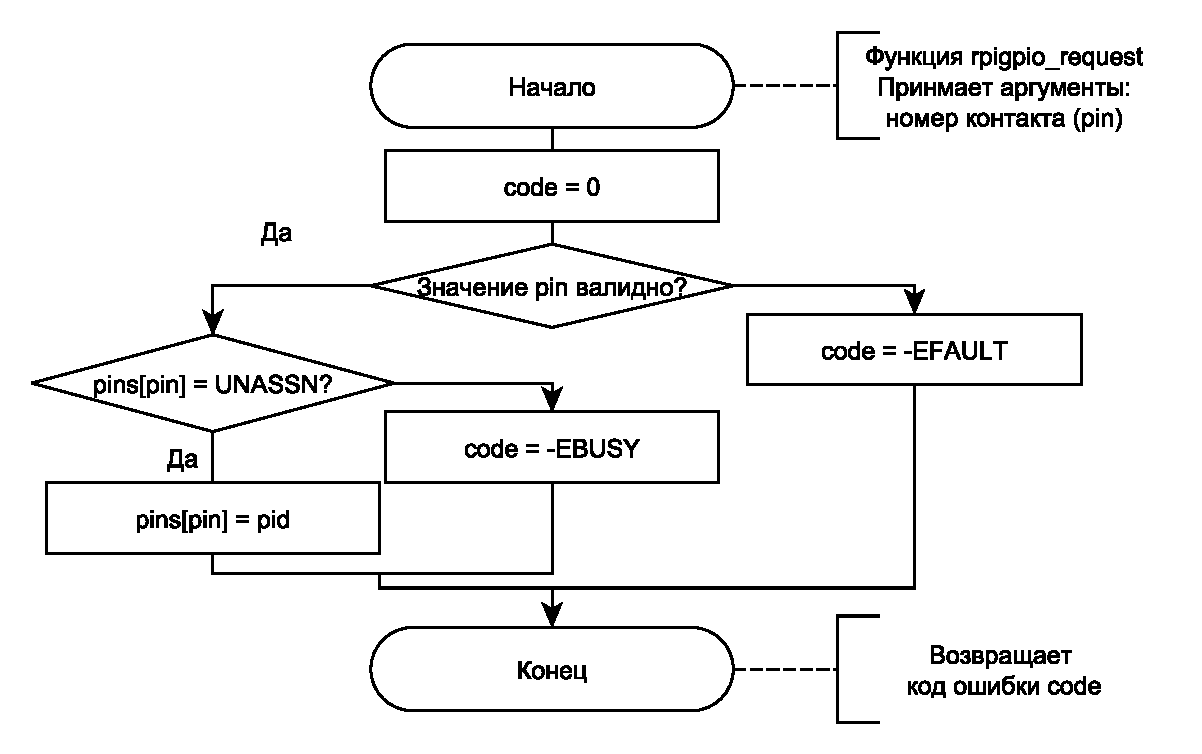
\includegraphics[scale=0.7, angle=0]{img/request.pdf}}
		\caption{Алгоритм захвата управления}
		\label{alg:request}
	\end{center}
\end{figure}

\begin{figure}[h!] 
	\begin{center}
		{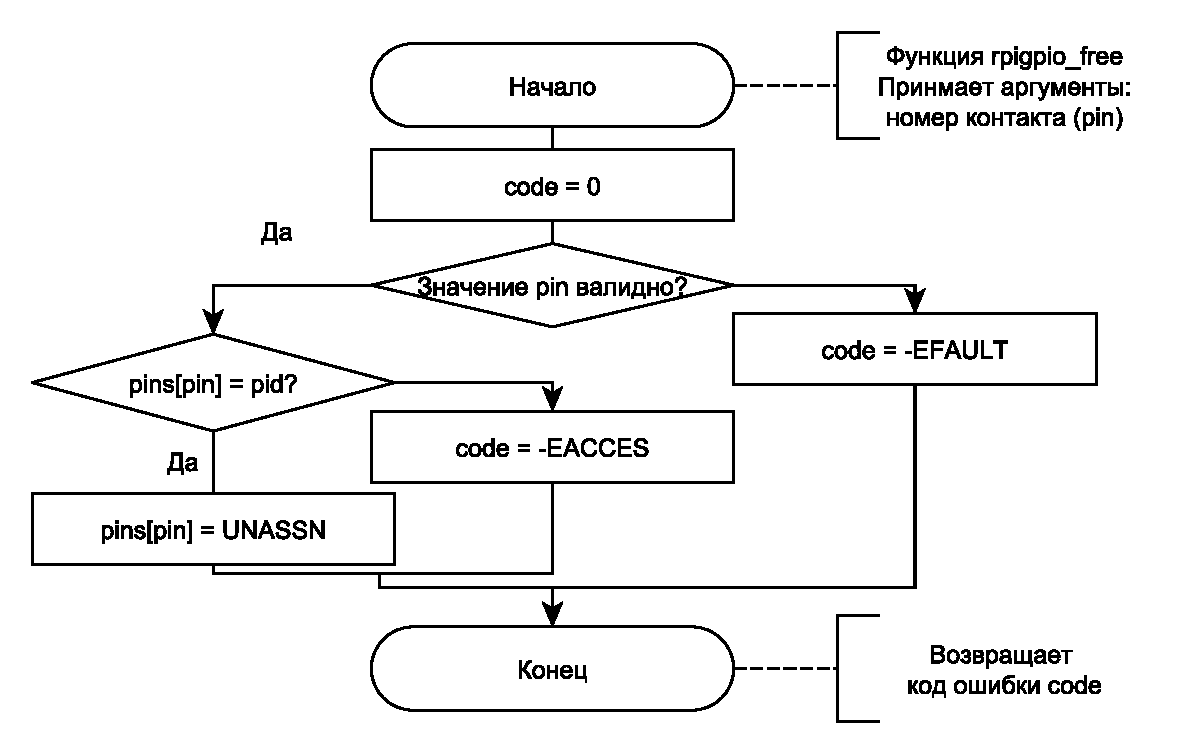
\includegraphics[scale=0.7, angle=0]{img/free.pdf}}
		\caption{Алгоритм возвращения управления}
		\label{alg:free}
	\end{center}
\end{figure}

\subsection{Алгоритмы установления режима работы}
На рисунке \ref{alg:mode} приведён алгоритм установления режима работы контакта.

\begin{figure}[h!] 
	\begin{center}
		{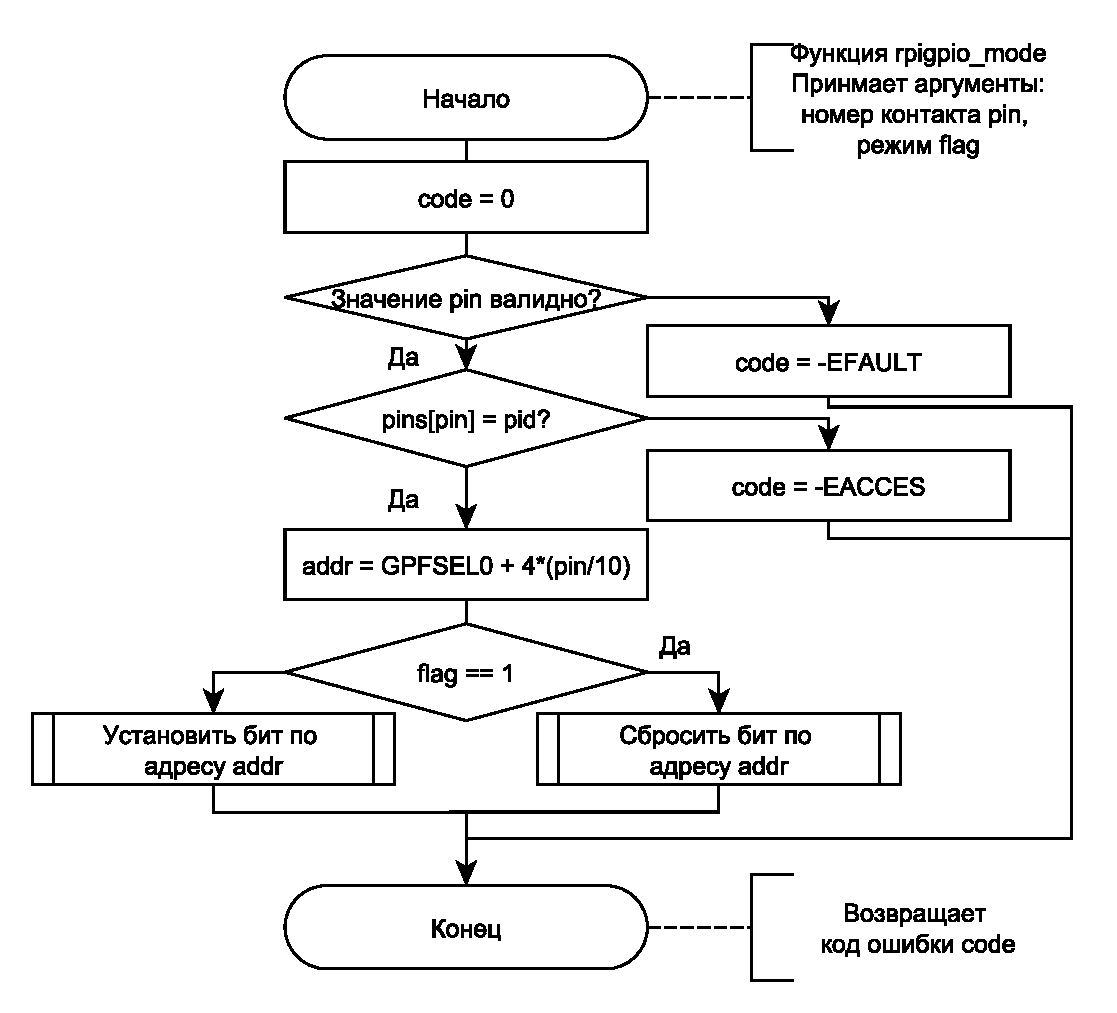
\includegraphics[scale=0.7, angle=0]{img/mode.pdf}}
		\caption{Алгоритм установления режима работы}
		\label{alg:mode}
	\end{center}
\end{figure}

\pagebreak